\documentclass[10pt]{amsart}
\usepackage{amsmath,amsthm,amssymb,amsfonts,enumerate,mymath,tikz-cd,pbox,mathtools}
\openup 5pt
\author{Blake Farman\\University of South Carolina}
\title{Math 788p:\\Homework 04}
\date{February 27, 2013}
\pdfpagewidth 8.5in
\pdfpageheight 11in
\usepackage[margin=1in]{geometry}

\begin{document}
\maketitle

\providecommand{\p}{\mathfrak{p}}
\providecommand{\m}{\mathfrak{m}}
\newcommand{\legendre}[2]{\left(\frac{#1}{#2}\right)}
\theoremstyle{plain}
\newtheorem{thm}{}
\newtheorem{lem}{Lemma}
\theoremstyle{definition}
\newtheorem{defn}{Definition}

\setcounter{thm}{7}

\begin{thm}
  Let $m$ and $n$ be distinct square-free integers not equal to 1.
  
  \begin{enumerate}[(a)]
  \item
    Prove that $\Q(\sqrt{m}, \sqrt{n})$ is Galois over $\Q$ with Galois group $\Z/2 \times \Z/2$.
    Does this field have any quadratic subfields other than $\Q(\sqrt{m})$ and $\Q(\sqrt{n})$.
  \item
    Suppose $p$ ramifies in both $\Q(\sqrt{m})$ and $\Q(\sqrt{n})$.
    What happens in $K$?
    Find an example.
  \item
    Suppose $p$ splits in both of these fields.
    What happens in $K$?
    Find an example.
  \item
    Suppose $p$ is inert in both of these fields.
    What happens in $K$?
    Find an example.
  \item
    Suppose the splitting behavior of $p$ is different in both of these fields.
    What happensi n $K$?
    Find an example.
  \item
    Does there exist an irreducible polynomial which is reducible mod every prime?
  \end{enumerate}
  
  \begin{proof}
    Let $K_1 = \Q(\sqrt{m})$ and $K_2 = \Q(\sqrt{n})$.
    \begin{enumerate}[(a)]
      \item
        First observe that $K$ is the splitting field for the polynomial $(x - m)(x + m)(x - n)(x + n)$ and thus is Galois over $\Q$.
        Provided $m \neq n$, this is a degree four extension of $\Q$.
        To see this, it suffices to show that $\sqrt{n} \not \in K_1$, for then $K = K_1(\sqrt{n})$ is a degree 2 extension of $K_1$.
        Assume to the contrary that $\sqrt{n} \in K_1$.
        Since $\sqrt{n}$ is integral over $\Z$, $\sqrt{n}$ would lie in $\mathcal{O}_{K_1}$.
        Hence there would exist integers $a$ and $b$ such that $\sqrt{n} = a + b\sqrt{m}$.
        Squaring both sides we have $n = a^2 + mb^2 + 2ab\sqrt{m}$.
        Since $\mathcal{B} = \left\{1, \sqrt{m}\right\}$ is an integral basis for $\mathcal{O}_{K_1}$ and $n = n + 0\sqrt{m}$, it follows that $ab = 0$, so at least one of $a,b$ is zero.
        However, this is absurd.
        If $b = 0$, then $n = a^2$, whereas $n$ was assumed to be square-free, a contradiction.
        Similarly, if $a = 0$, then $n/m = b^2$, also a contradiction since even if $m$ divides $n$, both $m$ and $n$ are square-free.
        Therefore $\Q(\sqrt{m}, \sqrt{n})$ is a degree four extension.
        
        To see that $\Gal{K/\Q} \cong \Z/2 \times \Z/2 \cong V_4$, observe that the identity and the following three involutions give all the automorphisms of $K$:
        $$
        \begin{array}{ccc}
          \sigma : \left\{
          \begin{array}{l}
            \sqrt{m} \mapsto \sqrt{m}\\
            \sqrt{n} \mapsto -\sqrt{n}
            \end{array}
          \right.
          &
          \tau : \left\{
          \begin{array}{l}
            \sqrt{m} \mapsto -\sqrt{m}\\
            \sqrt{n} \mapsto \sqrt{n}
            \end{array}
          \right.
        &
        \sigma\tau = \tau\sigma : \left\{
          \begin{array}{l}
            (\sqrt{m} \xmapsto{\tau} -\sqrt{m} \xmapsto{\sigma} -\sqrt{m}) = (\sqrt{m} \xmapsto{\sigma} \sqrt{m} \xmapsto{\tau} -\sqrt{m})\\
            (\sqrt{n} \xmapsto{\tau} \sqrt{n} \xmapsto{\sigma} -\sqrt{n}) = (\xmapsto{\sigma} -\sqrt{n} \xmapsto{\tau} -\sqrt{n}).
            \end{array}
          \right.\\
          \end{array}
        $$
        If $\ell = mn/(m,n)^2$, then it is clear from 
        $$\sigma\tau(a + b\sqrt{\ell}) = a + n\frac{\sigma\tau(\sqrt{m})\sigma\tau(\sqrt{n})}{(m,n)^2} = a + b\frac{(-\sqrt{m})(-\sqrt{n})}{(m,n)^2} = a + b\sqrt{\ell}$$
        that $K^{\left<\sigma\tau\right>} = \Q(\sqrt{\ell})$.
        Hence the subfields are given below
        \begin{center}
          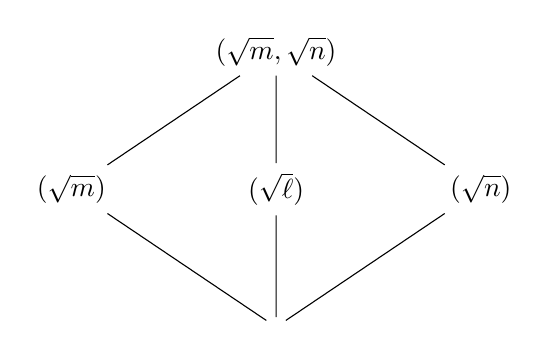
\begin{tikzpicture}[auto, xscale=.65, yscale=.35]
            \node(quart3) at (8,15){$\Q(\sqrt{m}, \sqrt{n})$};
            \node(quad1) at (4,10){$\Q(\sqrt{m})$};
            \node(quad2) at (8,10){$\Q(\sqrt{\ell})$};
            \node(quad3) at (12,10){$\Q(\sqrt{n})$};
            \node(q) at (8,5){$\Q$};
            \draw (quad1) to node {}(q);
            \draw (quad2) to node {}(q);
            \draw (quad3) to node {} (q);
            \draw (quad1) to node {} (quart3);
            \draw (quad2) to node {} (quart3);
            \draw (quad3) to node {} (quart3);
          \end{tikzpicture}
    \end{center}
      \item
        First observe that since $\Gal{K/\Q}$ is abelian, conjugation acts trivially and so there is exactly one decomposition group, $D$.
        Assume $p$ ramifies in $K_1$ and $K_2$.
        Note here that since the ramification index is multiplicative in towers, we have that $p$ does not split completely in $K$ and so $\abs{D} \geq 2$.
        Assume $p$ is odd and observe that $\ell$ is necessarily coprime to $m$ and $n$, so $p$ does not ramify in $K_3 = \Q(\sqrt{\ell})$.
        
        If $p$ splits in $K_3$, then it follows that $\abs{D} = 2$ and so $K^D$ is $K_3$.
        Hence $p = \p_1^2\p_2^2$ in $\mathcal{O}_K$.
        This occurs in the field $K = \Q(\sqrt{6}, \sqrt{10})$.
        The prime $5$ ramifies in the subfields $\Q(\sqrt{10})$ and $\Q(\sqrt{15})$ and splits in the subfield $\Q(\sqrt{6})$ as $(5, \sqrt{6} + 3)(5, \sqrt{6} + 2)$.
        In $K$, $(5) = (5, (\sqrt{6} + \sqrt{10}) + 1)^2(5, (\sqrt{6} + \sqrt{10}) - 1)^2$.
        
        If $p$ is inert in $K_3$, then it follows that $\abs{D} = 4$ and so $K^D$ is $\Q$.
        Since there is ramification in the two other subfields, it follows from multiplicativity of ramification indices and inertial degrees that $\abs{I} = 2$ and so $K^I = K_3$.
        Then $p = \p^2$ in $\mathcal{O}_K$ with $f(\p \mid p) = 2$.
        This occurs in the field $K = \Q(\sqrt{2}, \sqrt{3})$.
        In $\Q(\sqrt{3})$ and $\Q(\sqrt{6})$, 3 ramifies since it divides the discriminants, and remains inert in $\Q(\sqrt{2})$ since 2 is not a square modulo 3.
        In $K$, $(3) = (3, (\sqrt{2} + \sqrt{3})^2 + 1)^2$
        
        If $p = 2$, there are two cases.
        If $\ell \equiv 1 \pmod{4}$, then $2 \nmid \disc{K_3} = \ell$ and the cases are as above.
        However, if $\ell \equiv 3 \pmod{4}$, then $2 \mid \disc{K_3} = 4\ell$ and there is ramification in all three subfields.
        Then $D = 1$ and, since there is ramification in each of the subfields, $I = 1$.
        Hence $2$ is totally ramified in such cases.
        This occurs in $\Q(\sqrt{2}, \sqrt{3})$, with $(2) = (2, -1/2(\sqrt{2} + \sqrt{3}) + 1)$.
      \item
        Assume $p$ splits in $K_1$ and $K_2$.
        First note that $p \neq 2$ cannot ramify in $K_3$, for otherwise $p \mid \ell = mn / (m,n)^2$ implies $p$ divides exactly one of $m$ and $n$, and this cannot be since $p$ splits in $K_1$ and $K_2$.
        For $p = 2$, it follows that $m \equiv n \equiv 1 \pmod{4}$ (for otherwise 2 would ramify).
        Let $d = (m,n)$ so that $m = ad$ and $n = bd$ for some integers $a,b$.
        Then $a \equiv d \pmod{4}$ and $b \equiv d \pmod{4}$ force $\ell = ab \equiv d^2 \equiv 1 \pmod{4}$.
        Hence $p$ does not ramify in $K_3$.
        Similarly, $$\legendre{m}{p} = \legendre{a}{p}\legendre{d}{p} = 1 = \legendre{b}{p}\legendre{d}{p}= \legendre{n}{p}$$
        force $\legendre{\ell}{p} = 1$ and so $p$ splits in all three subfields.
        
        Assume that $\abs{D} = 2$ and let $\varphi \in \Gal{K/\Q}$ generate $D$.
        Let $\psi \in \Gal{K/\Q}$ be any other non-trivial automorphism.
        The primes of $\mathcal{O}_K$ lying above $p$ are $\p = \varphi(\p)$ and $\psi(\p) = \varphi\psi(\p)$.
        Let $H = \left<\psi\right>$ and consider the primes of $K^H$ lying over $\p$.
        Since $\psi$ fixes $K^H$, we have $\psi(\p) \cap K^H = \psi(\p \cap K^H) = \p \cap K^H$.
        Then by the observations above we now have
        $$\varphi(\p) \cap K^H = \p \cap K^H  = \psi(\p) \cap K^H = \varphi\psi(\p) \cap K^H,$$
        which is absurd since $p$ splits in all three subfields.
        Therefore $D = 1$ and $p$ splits completely.
        
        This occurs with $p = 23$ in the field $K = \Q(\sqrt{2}, \sqrt{3})$.
        In the subfields $\Q(\sqrt{2}), \Q(\sqrt{3}), \Q(\sqrt{6})$, 23 factors as $-(\sqrt{2} + 5)(\sqrt{2} - 5)$, $(3\sqrt{3} + 2)(3\sqrt{3} - 2)$, and $(2\sqrt{6} + 1)(2\sqrt{6} - 1)$, respectively.
        In $K$, we have the factorization 
        $$(23) = (23, (\sqrt{2} + \sqrt{3}) + 11), (23, (\sqrt{2} + \sqrt{3}) - 11), (23, (\sqrt{2} + \sqrt{3}) + 2), (23, (\sqrt{2} + \sqrt{3}) - 2).$$
      \item
        Assume $p$ is inert in $K_1$ and $K_2$.
        Note that by the same argument above, $p$ is not ramified in the third extension, and if $p = 2$, then $m \equiv n \equiv \ell \equiv 1 \pmod{4}$.
        For some integers $a,b$ and $d = (m,n)$, we have 
        $$\legendre{m}{p} = \legendre{a}{p}\legendre{d}{p} = -1 = \legendre{b}{p}\legendre{d}{p}= \legendre{n}{p}$$
        and so it must be the case that $\legendre{a}{p} = -\legendre{d}{p} = \legendre{b}{p}$, from which it follows that $\legendre{\ell}{p} = 1$ and $p$ splits in $K_3$.
        Hence it must be that $\abs{D} = 2$ and the factorization of $p$ in $K$ is $p = \p\p^\prime$ with $f(\p \mid p) = f(\p^\prime \mid p) = 2$.
        This occurs for $p = 5$ in $\Q(\sqrt{2}, \sqrt{3})$, which is inert in $K_1$ and $K_2$.
        In $K_3 = \Q(\sqrt{6})$, 5 splits as $5 = (\sqrt{6} + 1)(\sqrt{6} - 1)$.
        In $K$, we have $(5) = (5, (\sqrt{2} + \sqrt{3})^2 + 7), (5, (\sqrt{2} + \sqrt{3})^2 - 2)$
      \item
        First assume that $p$ splits in one of the two subfields.
        By the argument in part (c), note that the $p$ cannot split in only two subfields.
        Hence the second splitting type determines the splitting type in the third field.
        Namely, $p$ is either split in one and ramified in the other two, or $p$ is split in one and inert in the other two.
        That is $p = \p^2{\p^\prime}^2$ or $p = \p\p^\prime$ with $f(\p \mid p) = f(\p^\prime \mid p) = 2$, respectively.
        
        Similarly, by the argument in (c), $p$ cannot ramify in only one subfield.
        Hence if $p$ ramifies in one and is either inert or split in the second, then $p$ ramifies in the third subfield and the splitting types are $p = \p^2$ with $f(\p \mid p) = 2$ or $p = \p^2\p^2$, respectively.
      \item
        Yes: the irreducible polynomial $x^4 + 1$ is reducible modulo every prime $p$.
        If $p = 2$, then 
        $$x^4 + 1 = x^4 + 1^4 \equiv (x + 1)^4 \pmod{2}.$$
        If $p$ is odd, observe that $p^2 - 1$ is divisible by 8 since $p \equiv 1, 3, 5, 7 \pmod{8}$ and $1^2 \equiv 3^2 \equiv 5^2 \equiv 7^2 \equiv 1 \pmod{8}$.
        Let $p^2 - 1 = 8k$ for some integer $k$.
        Consider the polynomial $x^{p^2 - 1} - 1$.
        Writing $X = x^8$, it follows from $x^{p^2 - 1} - 1 = X^k - 1 = (X - 1)(X^{k - 1} + X^{k - 2} + \ldots + 1)$ that $x^8 - 1 = (x^4 + 1)(x^4 - 1)$ divides the polynomial $x^{p^2 - 1} - 1$, which in turn divides $x^{p^2} - x$.
        Regarding $\F_{p^2}$ as the splitting field of the latter polynomial, it follows that all the roots of $x^4 + 1$ lie in $\F_{p^2}$ and so have degree at most $2$ over $\F_p$.
        Therefore $x^4 + 1$ cannot be irreducible modulo $p$.
    \end{enumerate}
    
  \end{proof}
\end{thm}
\end{document}
